\documentclass[12pt]{article}
 
\usepackage{amssymb,amsfonts,amsmath}
\usepackage{bm}
\usepackage{dsfont}
\usepackage{color,soul}
\usepackage{graphicx}
\usepackage{caption}

\usepackage{float}
\usepackage{hyperref}

\usepackage{tikz}
\usetikzlibrary{backgrounds,fit,decorations.pathreplacing,calc}

\newcommand{\ket}[1]{\ensuremath{\left| #1 \right \rangle}}
\newcommand{\bra}[1]{\ensuremath{\left \langle #1 \right |}}
\newcommand{\braket}[2]{\ensuremath{\left\langle #1\left|#2 \right.\right\rangle}}
\def\ketbra#1#2{{\vert#1\rangle\!\langle#2\vert}}

\newcommand{\1}[1]{\mathds{1}\left[#1\right]}
\DeclareMathOperator{\Tr}{Tr}

\newtheorem{remark}{Remark}
\newtheorem{definition}{Definition}
\newtheorem{theorem}{Theorem}
\newtheorem{lemma}{Lemma}
\newtheorem{example}{Example}

\usepackage{bbm}

\newcommand{\eye}{\mathds{1}} % vector space identity op
\usepackage[dvipsnames]{xcolor}
\usepackage[colorinlistoftodos,textsize=small,backgroundcolor=BlueGreen,linecolor=Blue]{todonotes}


\title{Factoring $k$-controlled-unitaries into $4k^2$ controlled gates without ancillas}
\date{\today}

\author{Jacob Biamonte$^1$, Nike Dattani$^2$ and Mauro E.S.~Morales$^1$\\$^1$Deep Quantum Labs\\ Skolkovo Institute of Science and Technology\\ 3 Nobel Street, 
Moscow, Russia 121205\\
$^2$HPQC Labs \\ National Research Council of Canada \\ 100 Sussex Drive, Ottawa, Canada K1A 0R6}

%\homepage{DeepQuantum.AI}

\begin{document}
\maketitle

\subsection{The naive approach}

\begin{itemize}
    \item $12(k-1)$ 2-qubit gates, 
    \item $18(k-1)$ 1-qubit gates, 
    \item $k-1$ auxiliary qubits
    
\end{itemize}

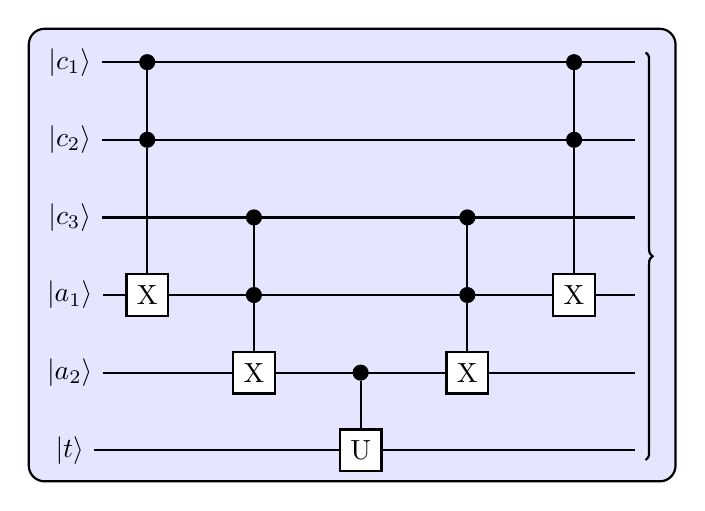
\begin{tikzpicture}[thick]
    % `operator' will only be used by Hadamard (H) gates here.
    % `phase' is used for controlled phase gates (dots).
    % `surround' is used for the background box.
    \tikzstyle{operator} = [draw,fill=white,minimum size=1.5em] 
    \tikzstyle{phase} = [draw,fill,shape=circle,minimum size=5pt,inner sep=0pt]
    \tikzstyle{surround} = [fill=blue!10,thick,draw=black,rounded corners=2mm]
    %
    \matrix[row sep=0.4cm, column sep=0.8cm] (circuit) {
    % First row.
    \node (q1) {\ket{c_1}}; &[-0.5cm] 
    \node[phase] (P11) {} ; & & & &
    \node[phase] (P16) {} ;&[-0.3cm]
    \coordinate (end1); \\
    % Second row.
    \node (q2) {\ket{c_2}}; &
    \node[phase] (P21) {}; & & & & 
    \node[phase] (P26) {} ;&
    \coordinate (end2);\\
    % Third row.
    \node (q3) {\ket{c_3}}; & & 
    \node[phase] (P32) {};  & &
    \node[phase] (P34) {};& 
    & 
    \coordinate (end3); \\
    % Fourth row.
    \node (q4) {\ket{a_1}}; &
    \node[operator] (X41) {X}; &
    \node[phase] (P42) {};  & &
    \node[phase] (P44) {}; &
    \node[operator] (X46) {X}; &
    \coordinate (end4); \\
    % Fifth row.
    \node (q5) {\ket{a_2}}; & &
    \node[operator] (X52) {X};  &
    \node[phase]    (P53) {};&
    \node[operator] (X54) {X};&&
    \coordinate (end5); \\
    % Sixth row.
    \node (q6) {\ket{t}}; & & &
     \node[operator] (U) {U};   & & &;
    \coordinate (end6); \\
    };
    % Draw bracket on right with resultant state.
    \draw[decorate,decoration={brace},thick]
        ($(circuit.north east)-(0cm,0.3cm)$)
        to node[midway,right] (bracket) {}
        ($(circuit.south east)+(0cm,0.3cm)$);
    \begin{pgfonlayer}{background}
        % Draw background box.
        \node[surround] (background) [fit = (q1) (U) (bracket)] {};
        % Draw lines.
        \draw[thick] (q1) -- (end1)  (q2) -- (end2) (q3) -- (end3) (q4) -- (end4) (q5) -- (end5) (q6) -- (end6) (P11) -- (P21) (P21) -- (X41)  (P32) -- (P42) (P42) -- (X52) (P53) -- (U) (P16) -- (P26) (P26) -- (X46) (P34) -- (P44) (P44) -- (X54);
    \end{pgfonlayer}
    %
    \end{tikzpicture}


\bibliography{refs}
\bibliographystyle{plain}
\end{document}